\begin{titlingpage}
  \begin{center}
    \vspace*{1in}

    \textbf{\large CS495\\ Optimiztaion}

    \vspace*{1in}

    Waleed A. Yousef, Ph.D.,

    \bigskip

    Human Computer Interaction Lab.,\\Computer Science Department,\\Faculty of Computers and
    Information,\\Helwan University,\\Egypt.

    \bigskip

    \today

  \end{center}
\end{titlingpage}

\clearpage

\hfil\begin{minipage}[t]{0.3\linewidth}
  Lectures follow \cite{Boyd204ConvexOptimization}:

  \bigskip

  \hfil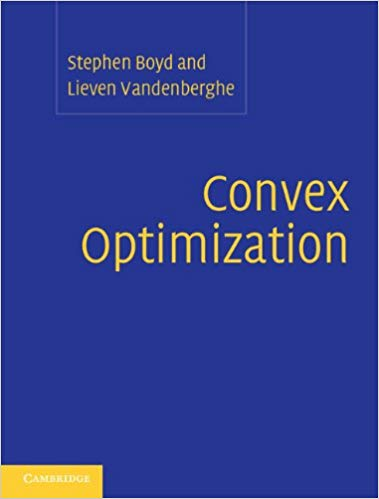
\includegraphics[height=0.5\textheight]{../Graphics/FrontCover1.png}\hfil

  Boyd, S., \& Vandenberghe, L. (2004). Convex Optimization. Cambridge: Cambridge University Press.

  \bigskip

  Book and Stanford course: \url{http://web.stanford.edu/~boyd/cvxbook/}

\end{minipage}\hfil
\begin{minipage}[t]{0.3\linewidth}
  Some examples from \cite{Chong2001AnIntorductionToOptimization}:

  \bigskip

  \hfil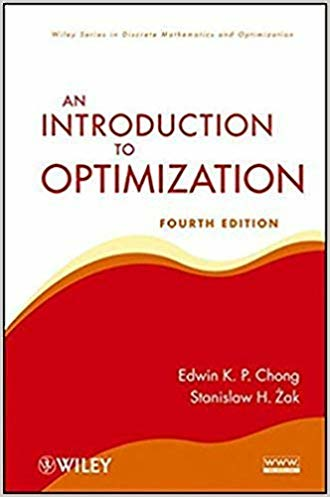
\includegraphics[height=0.5\textheight]{../Graphics/FrontCover2.png}\hfil

  Chong, E. K., \& Zak, S. (2001). An introduction to optimization: Wiley-Interscience.
\end{minipage}

\clearpage
\chapter*{Course Objectives}

\begin{itemize}
  \item Developing rigorous mathematical treatment for mathematical optimization.

  \item Building intuition, in particular to practical problems.

  \item Developing computer practice to using optimization SW.

\end{itemize}


\section*{Prerequisites}\label{cha:prerequisites}

Calculus (both single and multivariable) and Linear Algebra.

\clearpage
{
  \tiny
  \settocdepth{subsection}
  \tableofcontents
}

%%% Local Variables:
%%% mode: latex
%%% TeX-master: "../LectureNotes-Optimization"
%%% End:
